%%%%%%%%%%%%%%%%%%%% author.tex %%%%%%%%%%%%%%%%%%%%%%%%%%%%%%%%%%%
%
% sample root file for your "contribution" to a contributed volume
%
% Use this file as a template for your own input.
%
%%%%%%%%%%%%%%%% Springer %%%%%%%%%%%%%%%%%%%%%%%%%%%%%%%%%%


% RECOMMENDED %%%%%%%%%%%%%%%%%%%%%%%%%%%%%%%%%%%%%%%%%%%%%%%%%%%
\documentclass[graybox]{svmult}

% choose options for [] as required from the list
% in the Reference Guide

\usepackage{mathptmx}       % selects Times Roman as basic font
\usepackage{helvet}         % selects Helvetica as sans-serif font
\usepackage{courier}        % selects Courier as typewriter font
\usepackage{type1cm}        % activate if the above 3 fonts are
                            % not available on your system
%
\usepackage{makeidx}         % allows index generation
\usepackage{graphicx}        % standard LaTeX graphics tool
                             % when including figure files
\usepackage{multicol}        % used for the two-column index
\usepackage[bottom]{footmisc}% places footnotes at page bottom

% see the list of further useful packages
% in the Reference Guide

\makeindex             % used for the subject index
                       % please use the style svind.ist with
                       % your makeindex program

%%%%%%%%%%%%%%%%%%%%%%%%%%%%%%%%%%%%%%%%%%%%%%%%%%%%%%%%%%%%%%%%%%%%%%%%%%%%%%%%%%%%%%%%%

\begin{document}

\title*{Contribution Title}
% Use \titlerunning{Short Title} for an abbreviated version of
% your contribution title if the original one is too long
\author{Name of First Author and Name of Second Author}
% Use \authorrunning{Short Title} for an abbreviated version of
% your contribution title if the original one is too long
\institute{Name of First Author \at Name, Address of Institute, \email{name@email.address}
\and Name of Second Author \at Name, Address of Institute \email{name@email.address}}
%
% Use the package "url.sty" to avoid
% problems with special characters
% used in your e-mail or web address
%
\maketitle


\abstract{Each chapter should be preceded by an abstract (10--15 lines long) that summarizes the content. The abstract will appear \textit{online} at \url{www.SpringerLink.com} and be available with unrestricted access. This allows unregistered users to read the abstract as a teaser for the complete chapter. As a general rule the abstracts will not appear in the printed version of your book unless it is the style of your particular book or that of the series to which your book belongs.\newline\indent
Please use the 'starred' version of the new Springer \texttt{abstract} command for typesetting the text of the online abstracts (cf. source file of this chapter template \texttt{abstract}) and include them with the source files of your manuscript. Use the plain \texttt{abstract} command if the abstract is also to appear in the printed version of the book.}

\input{introduction}

\section{Planning acyclic contact sequences}
When planning the motion of a multiped robot, efficient
planners often rely on two simplifying assumptions:
firstly, the locomotion pattern is cyclic, and thus deterministic (when walking, after the left
foot the right foot always follows, and so on); secondly, the obstacles of the environment
can always be avoided in such a way that the first assumption is verified.

Discarding these assumptions is necessary for planning more complex motions.
For instance, for tasks such as standing up, climbing stairs
with a handrail, or getting out of a car, feasible solutions may require acyclic contact interactions between the robot and the environment.

However, acyclic contact planning requires 
handling a combinatorial, since any end effector can be used 
at any time, with any part of the environment. Moreover, the root path of the robot
must be computed at the same time as the contacts, adding a new layer of complexity~\citep{Bretl:2006:MPM:1124573.1124585, DBLP:conf/iser/EscandeKMG08}.

In this section, we describe a planner able to automatically compute 
a discrete sequence of contact configurations. These configurations verify a static equilibrium criterion,
and are used as an input guide path for the second step of our framework (Section TODO).

Contrary to previous contributions, the planner allows for \textit{interactive} performances.
This means that the next contact transition can be computed before the current contact transition
is executed on the robot. A pragmatic approach is chosen to break the combinatorial:
the planning of a root path is decoupled from the planning of the contacts.
First the planning of the root path is performed in a low dimensional space, which approximates 
the space of static equilibrium contact configurations (Section~\ref{sec:steve_root}).
Then a sequential algorithm is used to generate contacts along the computed path for the complete robot (Section~\ref{sec:steve_contact}).
As discussed in Section TODO decomposition results in a planner that can fail to compute a solution even if it exists.
However, experiments show that solutions can be effectively computed for various scenarios and robots, within seconds, where
complete systems can require up to hours of computation.

\subsection{Planning a root path}
\label{sec:steve_root}
In theory, decoupling the generation of a root path and contact configurations allows a strong 
reduction on the complexity of the acyclic contact planning problem, but raises a new scientific question: 
How to make sure that a root configuration allows to generate a contact configuration in static equilibrium?
We call such a root configuration an \textit{equilibrium feasible} configuration.
\cite{Bouyarmane2009} verify \textit{equilibrium feasibility} explicitly within their sampling based approach.
Because sampling a contact configuration is impossible (the contact manifold has a zero measure), when a root configuration is generated, a generalized inverse kinematics solver 
projects the robot onto a static equilibrium contact configuration. This is an expensive process, which prevents \textit{interactive} performances.

To avoid this explicit verification, we propose an inexpensive \textit{reachability condition}, drawn from an informal observation:
to create a contact with a surface, the root of the robot must be ``close, but not too close'': close enough
to allow contact creation; not too close to avoid colliding with the environment.
We then consider a dual representation to formulate this observation:
contact surfaces must lie in the reachable workspace of the robot limbs (Fig. TODO), and a scaling of the robot trunk must be collision free (Fig. TODO).
Given a parametrization, the condition defined by this representation is a trade-off between a necessary and a sufficient condition for the space of 
\textit{contact feasibile} root configurations, that is the space of root configurations which can lead to a contact.

To account for \textit{equilibrium feasibility} using the dual representation, we restrict our application domain.
We consider \textit{cluttered} problems, that admit as a solution a sequence of contact configurations for which at least one contact occurs with a surface whose friction cone contains the direction of the gravity (this includes all of the scenarios we mentionned).
For \textit{cluttered} problems, we assume \textit{equilibrium feasibility} is equivalent to \textit{contact feasibility}\footnote{We verify empirically this assumption in \cite{tonneauijrr16}}.

Under these assumptions, verifying that a root configuration is \textit{equilibrium feasible} requires a simple collision test thanks to the \textit{reachability condition}.
Therefore, to plan a root path for the robot, we can use any motion planner available from the litterature, such 
as the Bi-RRT planner \citep{770022}. With such a planner, restricting the configuration space of the robot to the low dimensional \textit{equilibrium feasible} space with the \textit{reachability condition} is trivial. We call our implementation of such a constrained planner RB-RRT, for \textit{Reachability-Based} RRT.

As an output of this phase, we obtain a continuous guide path of root configurations, assumed to be \textit{equilibrium feasible}.

\subsection{Generating contact configurations}
\label{sec:steve_contact}
The objective of this second phase is to extend a guide path for the root into a discrete sequence of full body, static equilibrium
contact configurations.

To achieve this, the input path is discretized, resulting in a list of root configurations.
The list is then traversed by the algorithm in an iterative fashion, starting from an input static equilibrium 
initial configuration. 

At each new step, an inverse kinematics solver tries to maintain all the contacts that existed in the previous step.
Contact failure can occur because of collisions or joint limit violation, in which case the contacts are invalidated.
Then, considering one contact free end-effector, a contact generator tries to generate a new contact that results in 
a static equilibrium configuration. If this fails, a new attempt is made with the next end-effector available, and so on.
Despite contact repositioning mechanisms to handle contact generation failure, the described algorithm can fail 
even if a feasible contact sequence exists. Again, this results from the trade-off made between efficiency and completeness, and empirical
results justify this approach. These statements are developed in in \cite{tonneauijrr16}.



\input{justin}

% !TEX root =  main.tex

% Chapter of 2-5 pages about torque ctrl, robust inv dyn and mujoco, 
% Use a high-level viewpoint, stressing the challenges of the proposed approach, almost no equation (similar to CR research project)
\section{Controlling the Motion on the Robot}
Once we have computed a trajectory of the CoM associated with a discrete sequence of contact configurations, we need to address the problem of how to execute this motion on a physical robot.
Clearly, different ways exist to tackle this problem.
Here we present the approach that we believe to be the best, and then we discuss the associated challenges and issues.

The main challenge when working on a real robot is the presence of uncertainties.
In the absence of uncertainties, planned motions could be directly executed on the robot.
Uncertainties make the robot deviate from the planned trajectories in unpredictable ways.
Our goal here is to react to these deviations (i.e. tracking errors) so as to get the robot to the desired final configuration without falling.

The specific features of legged robots make this task extremely hard.
First, these systems are subject to many constraints: motor torque and velocity bounds, joint position bounds, contact force friction cones, (self-)collisions.
This is clearly problematic because tracking errors may lead to constraint violations, which are typically connected to failure and damages of robot and/or environment.
Second, their dynamics is unstable and discontinuous (making/breaking contacts introduces discontinuities).
This means that small variations in control inputs or initial state may result in large variations of the future state.

\subsection{Model Predictive Control}
We believe that the best tool to control a constrained and unstable dynamical system is Model Predictive Control (MPC).
MPC consists in solving a discrete-time finite-horizon optimal control problem (OCP) and then using only the first part of the resulting control trajectory.
The process is repeated as fast as possible using the latest state estimation as initial state.
MPC has been successfully used for the control of chemical processes.
However, applications on legged robots are much more challenging:
\begin{itemize}
\item \textbf{High dimensionality}: solving an optimization problem is computationally demanding, especially when the size of state and control are large (around 60 for humanoids)
\item \textbf{Discontinuities}: the optimization process is slowed down by the discontinuities in the system dynamics, which need either to be approximated through smoothing~\citep{Todorov} or to be handled through hybrid models~\citep{Diehl2009a}.
\item \textbf{Non convexity}: the optimal control problem is not convex, so it needs to be properly initialized to converge to a \emph{``good-enough''} local minimum.
\end{itemize}
These challenges make it impossible to solve a new OCP at each sensor reading (typically every 1 ms) as we would like to. 
In practice we may only be able to do it every 10-100 sensor readings---which for a full humanoid still requires an extremely efficient implementation. 
In between two MPC computations we can still use the last-computed open-loop control trajectory.
In 2015 we reported the first application of whole-body nonlinear MPC on a humanoid robot (i.e. HRP-2)~\citep{Koenemann2015}.
\begin{figure}[!tbp]
\begin{center}
	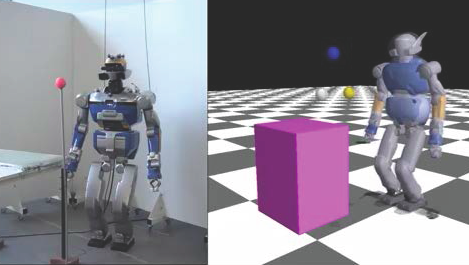
\includegraphics[width=0.4\textwidth]{figures/mujoco/ss0.png} \quad
	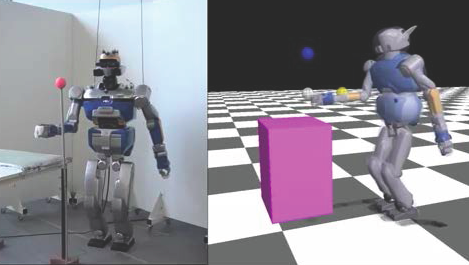
\includegraphics[width=0.4\textwidth]{figures/mujoco/ss1.png} \\
	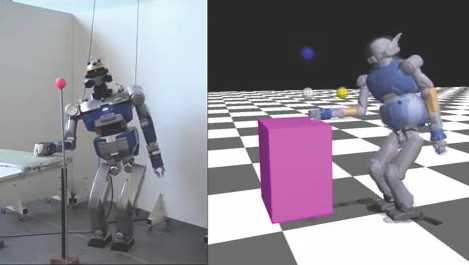
\includegraphics[width=0.4\textwidth]{figures/mujoco/ss2.png} \quad
	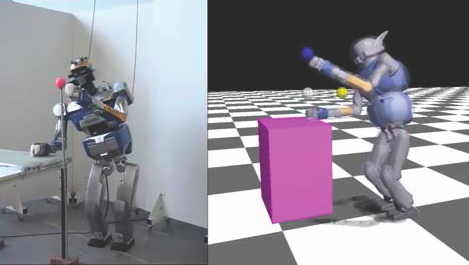
\includegraphics[width=0.4\textwidth]{figures/mujoco/ss3.png}
	\caption{Whole-body multi-contact experiment on HRP-2. The robot reaches for a target while it uses a table as an additional support to keep balance.}
	\label{fig:mujoco}
\end{center}
\end{figure}
To do that we used the efficient optimal-control framework MuJoCo~\citep{Todorov}, which can compute a 500ms trajectory for a 25-DoF robot in 50ms on a standard desktop computer.
Fig.~\ref{fig:mujoco} shows one of the experiments: HRP-2 reaches for a target making contact with a table for support.


\subsection{Constraint Robustness}
MPC inherently provides some level of robustness to uncertainties thanks to the frequent updates of the control trajectory based on the sensor feedback.
However, nothing prevents the solver to compute state-control trajectories that are close to the margins of their feasible sets.
When this happens, there is a high probability of violating some constraints, which often results in failure.
To solve this issue we can account for uncertainties in the OCP formulation, which leads us to \emph{Robust MPC}~\citep{Bemporad1999}.
While Robust MPC is an interesting and promising control paradigm, to the best of our knowledge it has never been used on legged robots.
The main reason is probably the computation time: in general Robust MPC is more computationally demanding than standard MPC, whose computation time is already the bottleneck for application on legged robots.

Despite this unpromising premise, the robotics community has recently started to study and apply robust control~\citep{Brasseur2015, Nguyen} and planning algorithms~\citep{Luo, Mordatch2015}.
In particular, we recently proposed an optimization-based inverse-dynamics control framework that tries to guarantee constraint satisfaction despite errors in the joint-torque tracking~\citep{DelPrete2015b}.
The accuracy of the torque tracking is known to be an important issue~\citep{Boaventura2012b, DelPrete2015a} (as we discuss at length in the next section), in particular for robots that do not have access to a direct measurement of the joint torques---such as most current humanoid robots: HRP-2, Hubo, Atlas, Valkyrie, Asimo, iCub. 
\begin{figure}[htbp]
   \centering
   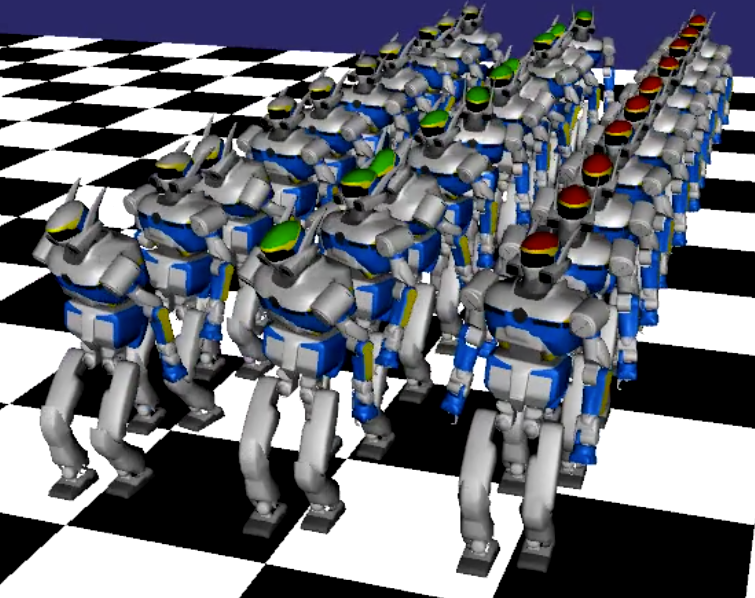
\includegraphics[width=0.5\textwidth]{figures/30_robots_walking.png} % requires the graphicx package
   \caption{Simulation of 30 HRP-2 robots walking in the presence of uncertainties, the goal being to compare the classic controller (left line) to the proposed robust controllers: stochastic (central line) and worst-case (right line).}
   \label{fig:robust_TSID}
\end{figure}
We validated the proposed methods on a simulated HRP-2 humanoid robot performing walking (see Fig. 1) and manipulation tasks, for which we presented statistics based on several batches of 100 tests each; in each batch we simulated different uncertainties.
We empirically showed that taking robustness into account greatly increases the chances of the robot not to fall, even in the presence of other uncertainties: velocity-estimation delays, inertial-parameter inaccuracies and limited actuator bandwidth. 
Moreover, we verified that we could solve the proposed optimization problems in less than 1 ms on a standard CPU, so that these formulations are suitable for online control.

Even if inverse-dynamics control is know to be more prone to myopic behaviors than MPC, these results encourage us to move forward towards Robust MPC.
However, the step from robust inverse dynamics to Robust MPC is not trivial and several concerns need to be addressed.
\begin{itemize}
\item Will the (likely) increased computation time be outweighed by the improved robustness?
\item Should we adopt an open-loop or a close-loop prediction scheme? In the presence of uncertainties, the classic open-loop prediction scheme used in MPC results in a pessimistic prediction of the future, which does not account for the fact that only the first value of the control trajectory is applied, and then the optimization is repeated using the new measurement. Open-loop prediction results then in too conservative behaviors, and close-loop prediction should be preferred. However, the latter results in an intractable optimization, which needs to be approximated---e.g. by assuming a linear feedback control law for the prediction.
\item Should we optimize performance for the nominal model or worst-case scenario? Considering the worst-case scenario leads to a minimax optimization that is in general much harder to solve; moreover, it can result in a too conservative behavior of the system.
\end{itemize}


\subsection{Joint Torque Control}
Another issue that we need to address for the real-robot implementation is the control of the actuators.
Typically whole-body control and planning assume joint torques as the control inputs.
However, real actuators are far from being the perfect torque source that we would like them to be.
This is due to the large friction in the transmission mechanisms (e.g. gear boxes, pistons).
Currently, the best solution seems to use joint-torque feedback~\citep{Albu-Schaffer2007, Boaventura2012b}.
Since in general this controller is not computationally demanding, it is better to decouple it from the whole-body MPC so as to run it at higher frequency (i.e. 1-3 kHz).

Despite being an essential component for the implementation of inverse-dynamics control, the problem of regulating the joint torques is still subject of ongoing research. The difference between the various works mainly lies in the type of actuator (rigid vs elastic, electric vs hydraulic) and the chosen actuator model (i.e. whether it includes the gear-box elasticity and/or the electric motor pole).

Our approach was to neglect the elasticity of the harmonic drive and the electric pole of the motor transfer function, which results in an instantaneous relationship between motor input and joint torque. 
While the model has experimentally proved to achieve a reasonable accuracy, it remarkably simplifies the identification procedure: in particular, we do not need to excite the robot at high frequencies. 
Most torque controllers rely on a direct measure of the joint torques. 
Since our robot is not equipped with joint-torque sensors, we estimate the joint torques using the procedure proposed for iCub~[4]: we propagate the wrenches measured by the F/T sensors (located at ankles and wrists) along the kinematic chain using a model of the dynamics of the robot and an estimation of velocities and accelerations of the robot bodies, reconstructed using the joint encoders and the IMU. 
This joint-torque estimation is used in the control to servo a feedback; it is also used offline to identify the relationship between the motor input and the associated joint torque. 
The torque-control law is a simple superposition of a feedforward term (given by the identified motor model) and a feedback term (based on the estimated joint torque). 
We validated the whole framework by implementing an inverse-dynamics controller on one leg of HRP-2, which has 6 joints. 
In comparison to the closed-source position control of HRP-2, we get a better position tracking while using lower feedback gains (up to 25\%). 
We also show the performances of our framework on a force-tracking task, which is easily integrated in the inverse-dynamics controller.


\input{sylvain}

\input{conclusion}

\bibliographystyle{plainnat}
\bibliography{references}
% %%%%%%%%%%%%%%%%%%%%%%%% referenc.tex %%%%%%%%%%%%%%%%%%%%%%%%%%%%%%
% sample references
% %
% Use this file as a template for your own input.
%
%%%%%%%%%%%%%%%%%%%%%%%% Springer-Verlag %%%%%%%%%%%%%%%%%%%%%%%%%%
%
% BibTeX users please use

%
\biblstarthook{References may be \textit{cited} in the text either by number (preferred) or by author/year.\footnote{Make sure that all references from the list are cited in the text. Those not cited should be moved to a separate \textit{Further Reading} section or chapter.} The reference list should ideally be \textit{sorted} in alphabetical order -- even if reference numbers are used for the their citation in the text. If there are several works by the same author, the following order should be used: 
\begin{enumerate}
\item all works by the author alone, ordered chronologically by year of publication
\item all works by the author with a coauthor, ordered alphabetically by coauthor
\item all works by the author with several coauthors, ordered chronologically by year of publication.
\end{enumerate}
The \textit{styling} of references\footnote{Always use the standard abbreviation of a journal's name according to the ISSN \textit{List of Title Word Abbreviations}, see \url{http://www.issn.org/en/node/344}} depends on the subject of your book:
\begin{itemize}
\item The \textit{two} recommended styles for references in books on \textit{mathematical, physical, statistical and computer sciences} are depicted in ~\cite{science-contrib, science-online, science-mono, science-journal, science-DOI} and ~\cite{phys-online, phys-mono, phys-journal, phys-DOI, phys-contrib}.
\item Examples of the most commonly used reference style in books on \textit{Psychology, Social Sciences} are~\cite{psysoc-mono, psysoc-online,psysoc-journal, psysoc-contrib, psysoc-DOI}.
\item Examples for references in books on \textit{Humanities, Linguistics, Philosophy} are~\cite{humlinphil-journal, humlinphil-contrib, humlinphil-mono, humlinphil-online, humlinphil-DOI}.
\item Examples of the basic Springer style used in publications on a wide range of subjects such as \textit{Computer Science, Economics, Engineering, Geosciences, Life Sciences, Medicine, Biomedicine} are ~\cite{basic-contrib, basic-online, basic-journal, basic-DOI, basic-mono}. 
\end{itemize}
}

\begin{thebibliography}{99.}%
% and use \bibitem to create references.
%
% Use the following syntax and markup for your references if 
% the subject of your book is from the field 
% "Mathematics, Physics, Statistics, Computer Science"
%
% Contribution 
\bibitem{science-contrib} Broy, M.: Software engineering --- from auxiliary to key technologies. In: Broy, M., Dener, E. (eds.) Software Pioneers, pp. 10-13. Springer, Heidelberg (2002)
%
% Online Document
\bibitem{science-online} Dod, J.: Effective substances. In: The Dictionary of Substances and Their Effects. Royal Society of Chemistry (1999) Available via DIALOG. \\
\url{http://www.rsc.org/dose/title of subordinate document. Cited 15 Jan 1999}
%
% Monograph
\bibitem{science-mono} Geddes, K.O., Czapor, S.R., Labahn, G.: Algorithms for Computer Algebra. Kluwer, Boston (1992) 
%
% Journal article
\bibitem{science-journal} Hamburger, C.: Quasimonotonicity, regularity and duality for nonlinear systems of partial differential equations. Ann. Mat. Pura. Appl. \textbf{169}, 321--354 (1995)
%
% Journal article by DOI
\bibitem{science-DOI} Slifka, M.K., Whitton, J.L.: Clinical implications of dysregulated cytokine production. J. Mol. Med. (2000) doi: 10.1007/s001090000086 
%
\bigskip

% Use the following (APS) syntax and markup for your references if 
% the subject of your book is from the field 
% "Mathematics, Physics, Statistics, Computer Science"
%
% Online Document
\bibitem{phys-online} J. Dod, in \textit{The Dictionary of Substances and Their Effects}, Royal Society of Chemistry. (Available via DIALOG, 1999), 
\url{http://www.rsc.org/dose/title of subordinate document. Cited 15 Jan 1999}
%
% Monograph
\bibitem{phys-mono} H. Ibach, H. L\"uth, \textit{Solid-State Physics}, 2nd edn. (Springer, New York, 1996), pp. 45-56 
%
% Journal article
\bibitem{phys-journal} S. Preuss, A. Demchuk Jr., M. Stuke, Appl. Phys. A \textbf{61}
%
% Journal article by DOI
\bibitem{phys-DOI} M.K. Slifka, J.L. Whitton, J. Mol. Med., doi: 10.1007/s001090000086
%
% Contribution 
\bibitem{phys-contrib} S.E. Smith, in \textit{Neuromuscular Junction}, ed. by E. Zaimis. Handbook of Experimental Pharmacology, vol 42 (Springer, Heidelberg, 1976), p. 593
%
\bigskip
%
% Use the following syntax and markup for your references if 
% the subject of your book is from the field 
% "Psychology, Social Sciences"
%
%
% Monograph
\bibitem{psysoc-mono} Calfee, R.~C., \& Valencia, R.~R. (1991). \textit{APA guide to preparing manuscripts for journal publication.} Washington, DC: American Psychological Association.
%
% Online Document
\bibitem{psysoc-online} Dod, J. (1999). Effective substances. In: The dictionary of substances and their effects. Royal Society of Chemistry. Available via DIALOG. \\
\url{http://www.rsc.org/dose/Effective substances.} Cited 15 Jan 1999.
%
% Journal article
\bibitem{psysoc-journal} Harris, M., Karper, E., Stacks, G., Hoffman, D., DeNiro, R., Cruz, P., et al. (2001). Writing labs and the Hollywood connection. \textit{J Film} Writing, 44(3), 213--245.
%
% Contribution 
\bibitem{psysoc-contrib} O'Neil, J.~M., \& Egan, J. (1992). Men's and women's gender role journeys: Metaphor for healing, transition, and transformation. In B.~R. Wainrig (Ed.), \textit{Gender issues across the life cycle} (pp. 107--123). New York: Springer.
%
% Journal article by DOI
\bibitem{psysoc-DOI}Kreger, M., Brindis, C.D., Manuel, D.M., Sassoubre, L. (2007). Lessons learned in systems change initiatives: benchmarks and indicators. \textit{American Journal of Community Psychology}, doi: 10.1007/s10464-007-9108-14.
%
%
% Use the following syntax and markup for your references if 
% the subject of your book is from the field 
% "Humanities, Linguistics, Philosophy"
%
\bigskip
%
% Journal article
\bibitem{humlinphil-journal} Alber John, Daniel C. O'Connell, and Sabine Kowal. 2002. Personal perspective in TV interviews. \textit{Pragmatics} 12:257--271
%
% Contribution 
\bibitem{humlinphil-contrib} Cameron, Deborah. 1997. Theoretical debates in feminist linguistics: Questions of sex and gender. In \textit{Gender and discourse}, ed. Ruth Wodak, 99--119. London: Sage Publications.
%
% Monograph
\bibitem{humlinphil-mono} Cameron, Deborah. 1985. \textit{Feminism and linguistic theory.} New York: St. Martin's Press.
%
% Online Document
\bibitem{humlinphil-online} Dod, Jake. 1999. Effective substances. In: The dictionary of substances and their effects. Royal Society of Chemistry. Available via DIALOG. \\
http://www.rsc.org/dose/title of subordinate document. Cited 15 Jan 1999
%
% Journal article by DOI
\bibitem{humlinphil-DOI} Suleiman, Camelia, Daniel C. O�Connell, and Sabine Kowal. 2002. `If you and I, if we, in this later day, lose that sacred fire...�': Perspective in political interviews. \textit{Journal of Psycholinguistic Research}. doi: 10.1023/A:1015592129296.
%
%
%
\bigskip
%
%
% Use the following syntax and markup for your references if 
% the subject of your book is from the field 
% "Computer Science, Economics, Engineering, Geosciences, Life Sciences"
%
%
% Contribution 
\bibitem{basic-contrib} Brown B, Aaron M (2001) The politics of nature. In: Smith J (ed) The rise of modern genomics, 3rd edn. Wiley, New York 
%
% Online Document
\bibitem{basic-online} Dod J (1999) Effective Substances. In: The dictionary of substances and their effects. Royal Society of Chemistry. Available via DIALOG. \\
\url{http://www.rsc.org/dose/title of subordinate document. Cited 15 Jan 1999}
%
% Journal article by DOI
\bibitem{basic-DOI} Slifka MK, Whitton JL (2000) Clinical implications of dysregulated cytokine production. J Mol Med, doi: 10.1007/s001090000086
%
% Journal article
\bibitem{basic-journal} Smith J, Jones M Jr, Houghton L et al (1999) Future of health insurance. N Engl J Med 965:325--329
%
% Monograph
\bibitem{basic-mono} South J, Blass B (2001) The future of modern genomics. Blackwell, London 
%
\end{thebibliography}

\end{document}
